\chapter{Analysis and Conclusions}
\label{analysis}

% answer subquestion one: what patterns can be found using wavelet analysis?
\section{Wavelet analysis}
In verification of Hypothesis \ref{hyp:subsequent_data}, the requirement of a
subsequent data series for wavelet analysis, a hypothetical signal was
constructed. Let the following set of pairs be the signal $S$ to be analysed,
where the first value is the time value, and the second value the LOC value:
$$S = \{(1,100), (2,150), (5,250)\}$$

\noindent
In signal $S$ the two pairs between $(2,150)$ and $(5,250)$ are missing. The
implementation of discrete wavelet transform in the 'wavelets' R package
requires an indexed series as input wavelet. This means, that whether or not
the signal contains gaps, these gaps are automatically closed by using a
subsequent index. After indexing, the signal $S$ will look as follows:
$$S' = \{(0,100), (1,150), (2,250)\}$$

\noindent
The wavelet transformation can perfectly be done by using $S'$ as input
signal and the output series of coefficients are indistinguishable from a
signal without gaps. However, the patterns that are found will be invald as it
was found by ignoring the missing data.

\paragraph{}
A further investigation was done on how to fix such gaps, using three different
methods of 'guessing' the data:
\begin{description}
	\item[last observation carried] \hfill \\[1em]
	$\grave{S}' = \{(1,100), (2,150), (3,150), (4,150), (5,250)\}$

	\item[mean] \hfill \\[1em]
	$\grave{S}'' = \{(1,100), (2,150), (3,200), (4,200), (5,250)\}$
	
	\item[piecewise constant interpolation] \hfill \\[1em]
	$\grave{S}''' = \{(1,100), (2,150), (3,150), (4,250), (5,250)\}$
	
	\item[linear interpolation] \hfill \\[1em]
	$\grave{S}'''' = \{(1,100), (2,150), (3,183), (4,216), (5,250)\}$
\end{description}

\paragraph{}
Using the first method \emph{last observation carried }\rm will give a signal
with a flat line between point 2 and 5. Filling the gap with \emph{mean }\rm
values, will still result in a signal with a flat line, although smaller, but
still undesired. The \emph{piecewise constant }\rm interpolation results in two
smaller flat lines. And the \emph{linear interpolation }\rm will give a signal
that will linearly flow towards the next known value. 

The flat lines, when it lasts long enough, may be detected as no change in LOC
during that period. This is undesired as can be mistaken for a pattern that
stopped code evolution.

However, the linear line could be mistaken for growth or shrink in LOC,
depending on the direction of the line. If the period of interpolation is long
enough, this also might give the wrong idea. Either way, 'guessing' missing data
adds noise. Not only to the project itself, but to the analysis as a whole.

\paragraph{}
The success of one of the above methods of closing a gap depends on the size of
the gap. The smaller the gap, the lesser impact it has on the reliability of
the detection of a pattern for that particluar signal. The larger the gap, the
more the impact on reliability. However, in general having gaps in the data
negatively influences the reliability of detecting patterns. Therefore,
Hypothesis \ref{hyp:subsequent_data} is confirmed.

\section{Sequence analysis}
There are more than 100,000 times more similar sequences found in the
scale/filter coefficients than in the wavelet/shift coefficients. The large
difference in number of sequences found between the two types of coefficients
is due to the fact that the LOC metric is a cumulative metric. The typical shape
of the LOC metric is a growing line. This makes finding a matching sequence of
coefficients using only shift coefficients (i.e., along the time axis) less
likely.

\paragraph{}
The fact that, of the 16,049 patterns, there are 0 patterns found in shift
coefficients was to be expected. The 16 similar sequences in shift coefficients
are not similar within the same group of sequences. Additionally, the shift
coefficients are incomparable to the filter coefficients because it is a
fundamentally different way of signal transformation. Mixing both types of
coefficients would ignore how the coefficients were found and invalidate the
patterns.

\section{Pattern analysis}
\label{section:pattern_evaluation}
To be able to know what the patterns represent, the 16,049 patterns are
projected onto the original signal. This is done by finding the project the
pattern was first detected, and taking the pattern's level of decomposition and
starting point in the series of coefficients for its project.

As the set of values of level of decomposition, starting point in the series,
its length (i.e., number of coefficients), and the originating project is
unique for each pattern, it can be 're-projected' onto the signal of that
particular project. This gives the $age\_in\_months$ values the sequence starts
and ends in the project.

Knowing the start and end month of a sequence within a project, the values of
the original signal during the sequence are captured for further analysis.

\paragraph{}
In verification of hypothesis \ref{hyp:pattern_low_diff}, the absolute maximum
differences of the LOC values is computed for each sequence. The patterns have
maximum LOC differences between 0 (i.e., no change in LOC in the sequence) and
6,862,111. Figure \ref{figure:pattern_loc_diff} shows the number of patterns
having a certain value of maximum LOC difference.

\begin{figure}[H]
\caption{Distribution of maximum LOC differences across
patterns}\label{figure:pattern_loc_diff}
\centering
	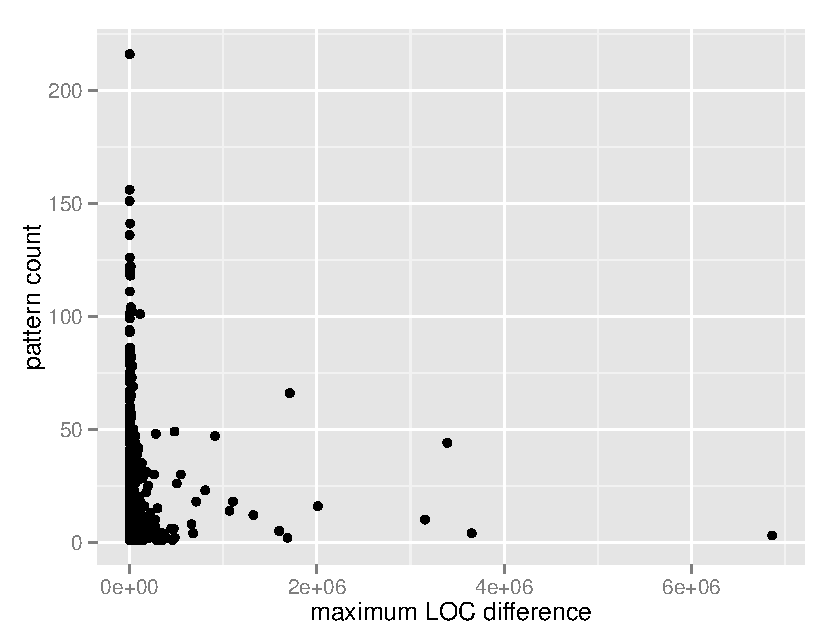
\includegraphics[width=296pt]{images/pattern_LOC_diff_100.pdf}
\end{figure}

\noindent
75\% of the patterns have a maximum LOC difference less than 20,595; 50\% have
a maximum LOC difference less than 5,250; and 25\% less than 1,046.

\subsection{Pattern type A}
The 25 type A patterns occur in 11 of the 21 dead projects. From the definition
of a type A pattern, it should occur strictly at the end of the evolution of a
dead project. This means that patterns overlap. At first, one would expect that
there could be only one pattern at the end of the evolution of the same
project. It appears there can be more than one. The patterns that overlap do
last until the end of the evolution of a project, but they can start earlier.

\paragraph{}
For the 25 patterns of type A, which occur at the end of evolution of dead
projects (section \ref{section:patterns_dead}), the maximum LOC differences are
distributed differently than for the set of patterns as a whole. Table
\ref{table:type_a_max_diff} shows the number of type A patterns having a
certain value of maximum LOC difference.

\newcommand{\tableHeadTypeALocDiff}{\bfseries{max. LOC diff.}\rm &
\bfseries{pattern count}\rm}
\begin{table}[H]
\caption{Maximum LOC difference of type A patterns}\label{table:type_a_max_diff}
\centering
\begin{tabular}{rr}
\hline
	\tableHeadTypeALocDiff \\
	\hline
   189 &   4 \\ 
  1404 &   3 \\ 
   42 &   2 \\ 
  1093 &   2 \\ 
  1242 &   2 \\ 
  13199 &   2 \\ 
  14112 &   2 \\ 
    0 &   1 \\
\hline
\end{tabular}
\begin{tabular}{rr}
\hline
  \tableHeadTypeALocDiff \\
  \hline 
   10 &   1 \\ 
  487 &   1 \\ 
  4263 &   1 \\ 
  5766 &   1 \\ 
  11930 &   1 \\ 
  13193 &   1 \\ 
  223157 &   1 \\
  \\ 
\hline
\end{tabular}
\end{table}

\noindent
Table \ref{table:type_a_max_diff} suggests that Hypothesis
\ref{hyp:pattern_low_diff} is \emph{false}\rm: it is not typically the case
that patterns in LOC at the end of code evolution of dead projects have a low
difference in LOC. The hypothesis is false in this data set.

\paragraph{}
The four patterns having the most common values of maximum LOC difference are
shown in Figure \ref{figure:top_patterns_plots} to illustrate how these look
like. The figure depicts the wavelets of the patterns, which are the LOC values
at a given snapshot in time for the dead project it was detected in.

\begin{figure}[H]
\caption{The four most common type A patterns projected onto original
signal}\label{figure:top_patterns_plots}
\centering
	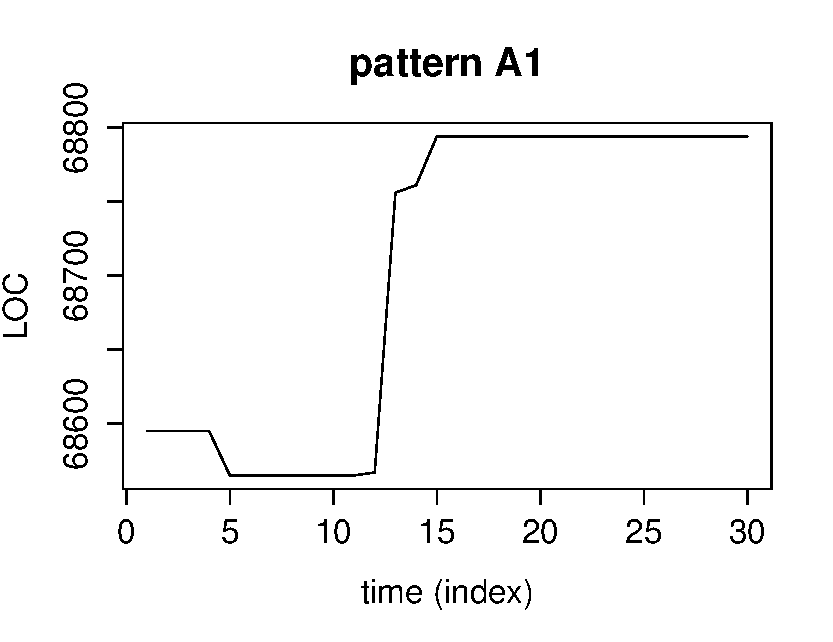
\includegraphics[width=196pt]{images/pattern_a1.pdf}
	\hspace{1em}
	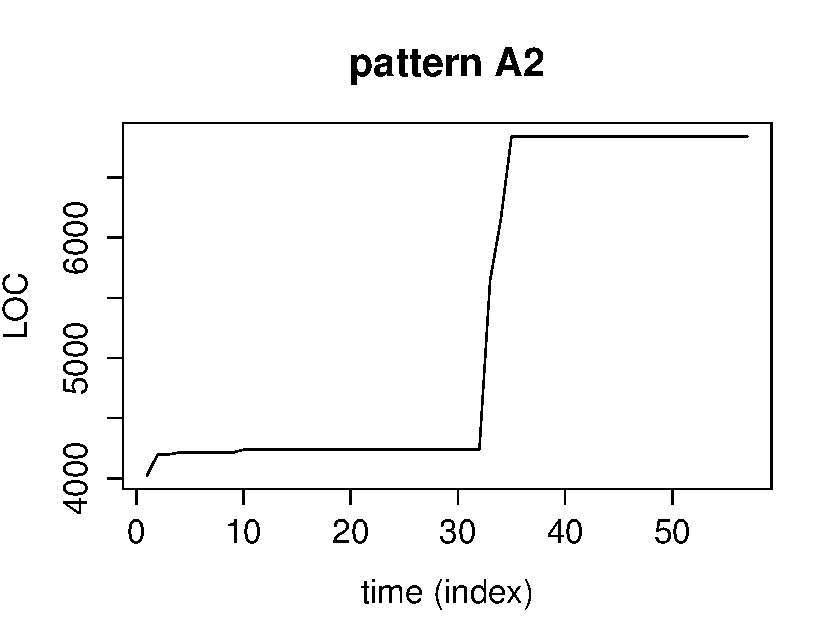
\includegraphics[width=196pt]{images/pattern_a2.pdf}
	\\
	\vspace{1em}
	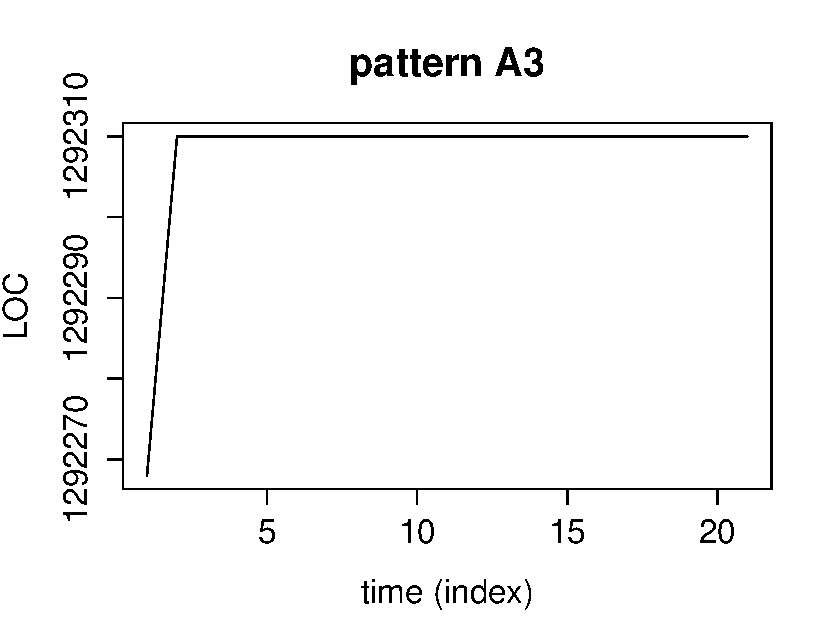
\includegraphics[width=196pt]{images/pattern_a3.pdf}
	\hspace{1em}
	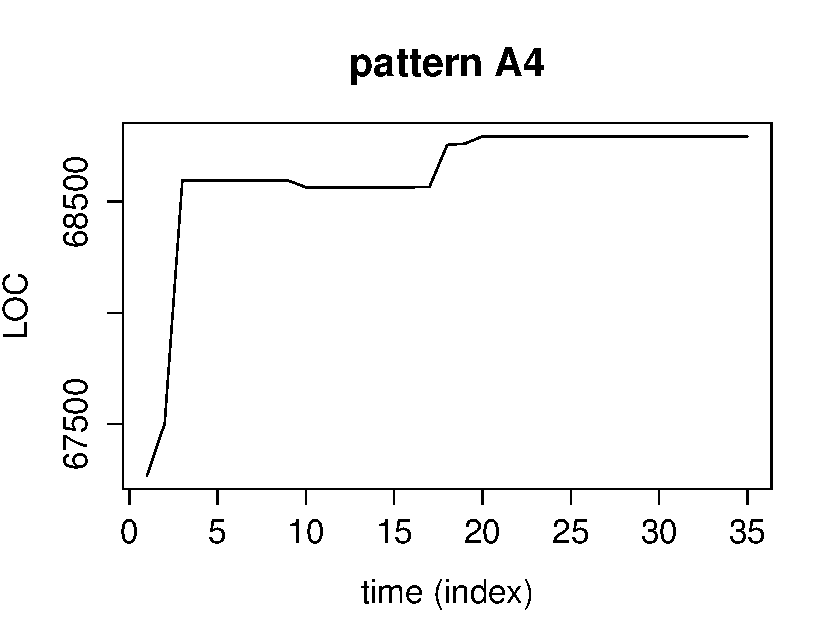
\includegraphics[width=196pt]{images/pattern_a4.pdf}
\end{figure}

\paragraph{}
Figure \ref{figure:top_patterns_plots} also show the lengths of the patterns.
The shortest pattern lasts 19 months, the longest 57. 75\% of the type A
patterns detected have a length of at least 25 months.

\subsection{Warning signs}
The type A patterns would be the best candidates for being 'warning signs' as
they are detected at the end of evolution in dead projects. After selection of
all the projects patterns of type A occur in, a total of 93 projects are found.
Of which 11 were already in the pool of dead projects, and 79 are 'alive'
projects.

Using this group of 93 projects having a type A pattern, a second group of 93
projects can be selected having not the pattern. This second group is
representative to the complete data set, again using the tool by
\citet{nagappan}. For each project of both groups it is recorded at what age the
project died, that is, if it died. For the others, the maximum age in the data
set is used. In Figure \ref{figure:kp_survival} the Kaplan-Meier estimation of
the survival function is shown for these groups.

\begin{figure}[H]
\caption{Kaplan-Meier estimation survival of projects regarding type A
patterns}\label{figure:kp_survival}
\centering
	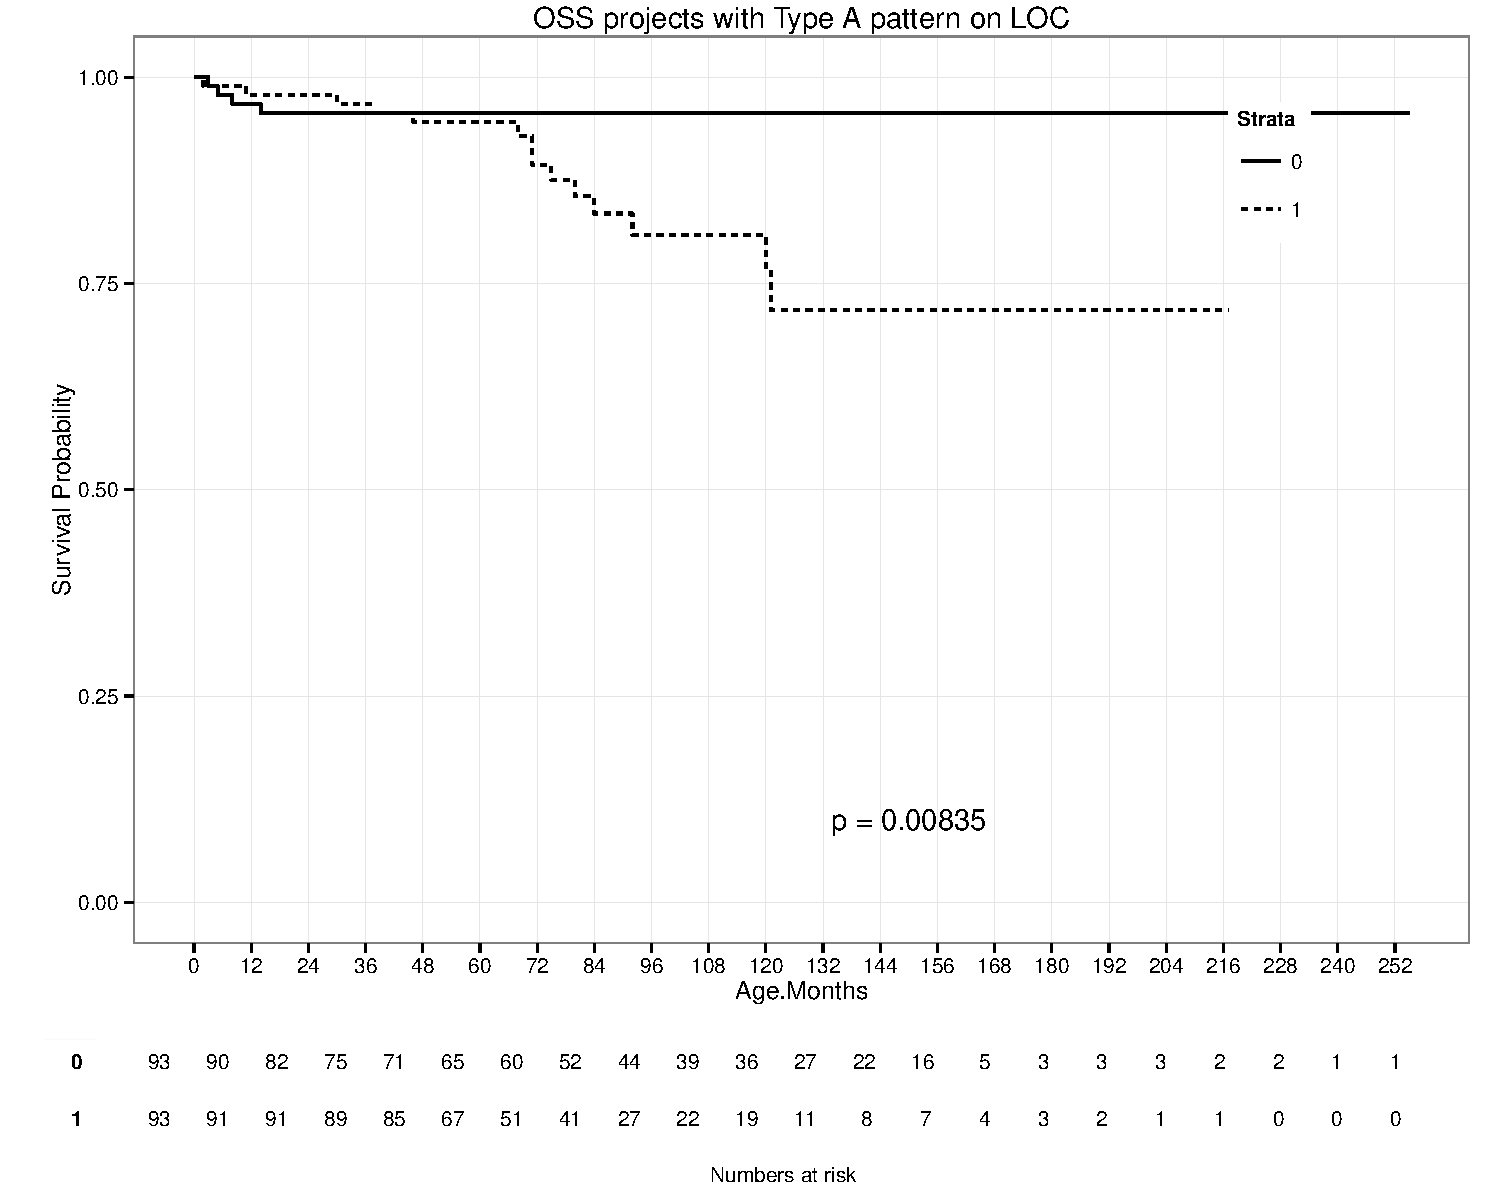
\includegraphics[width=386pt]{images/survival_LOC.pdf}
\end{figure}

\noindent
Figure \ref{figure:kp_survival} suggests that group 1 of projects having the
type A pattern die earlier than group 0 of projects without the pattern. This
suggests that having a type A pattern shortens the life of a project.

\begin{comment}
\paragraph{}
The four patterns with the most common maximum LOC differences are shown in
Figure \ref{figure:top_patterns_plots} to illustrate how such patterns look
like. The figure depicts the wavelets of the patterns for all the project
signals they were detected in. Which are the differences in LOC values between
two subsequent coefficients.

\begin{figure}[H]
\caption{The four most common type A patterns projected onto original
signal}\label{figure:top_patterns_plots}
\centering
	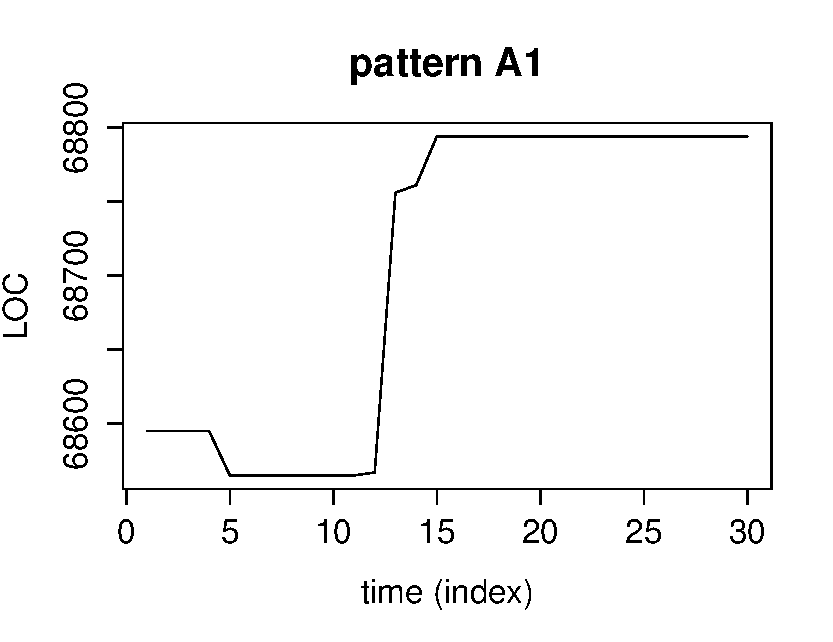
\includegraphics[width=196pt]{images/pattern_a1.pdf}
	\hspace{1em}
	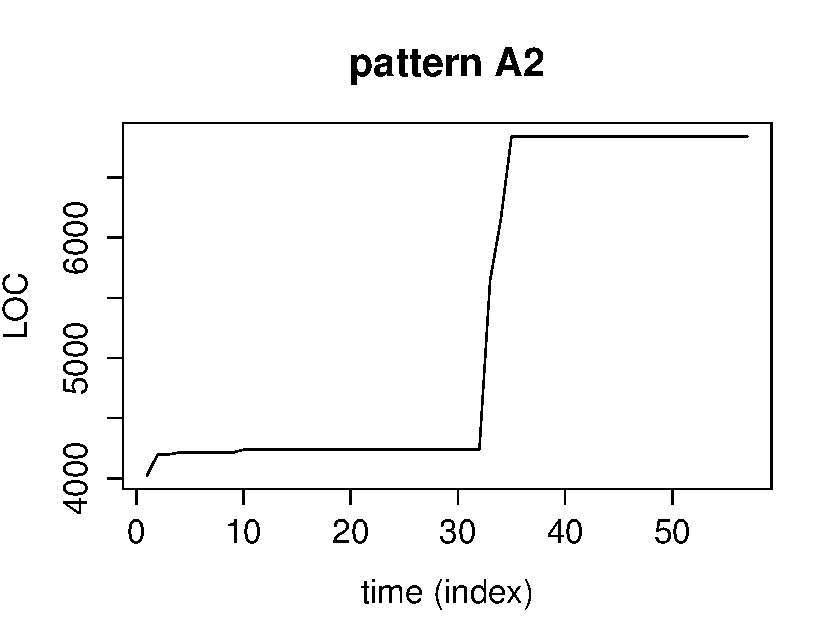
\includegraphics[width=196pt]{images/pattern_a2.pdf}
	\\
	\vspace{1em}
	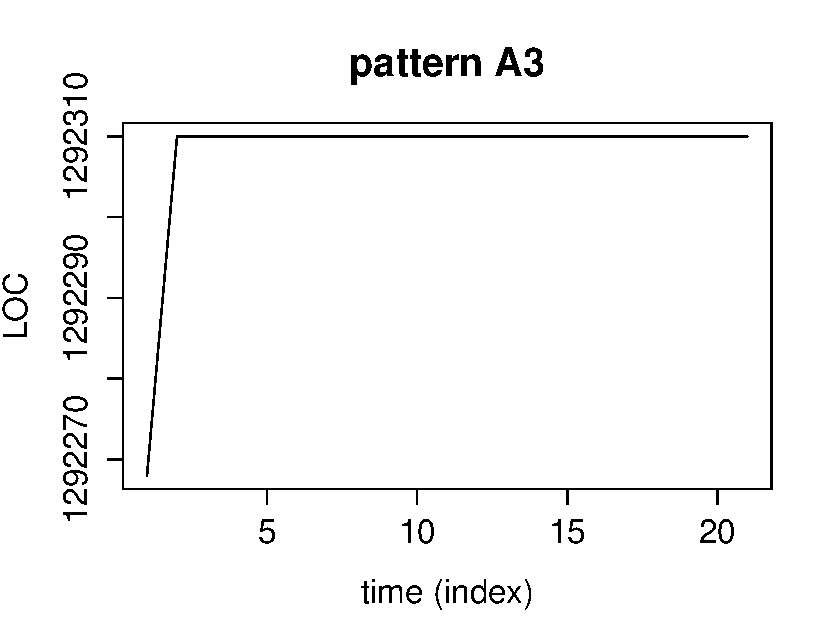
\includegraphics[width=196pt]{images/pattern_a3.pdf}
	\hspace{1em}
	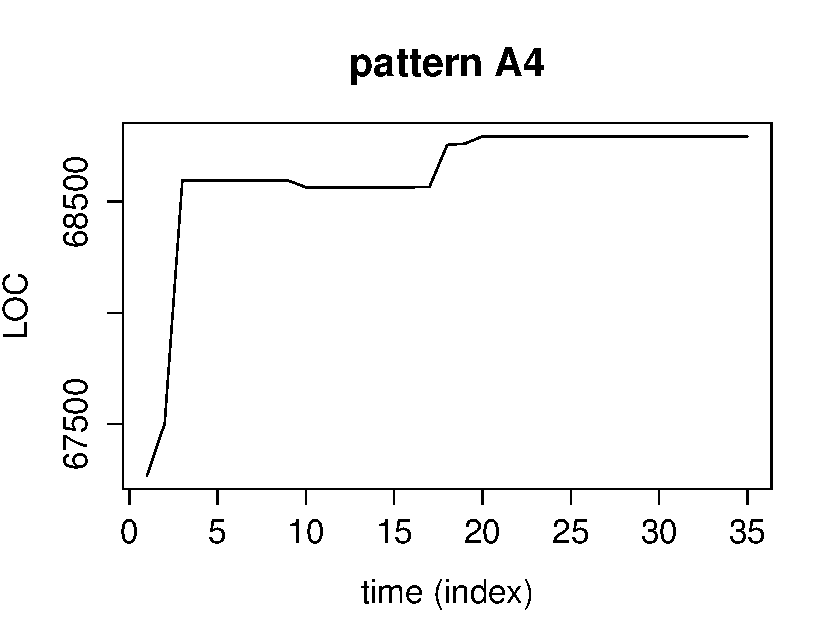
\includegraphics[width=196pt]{images/pattern_a4.pdf}
\end{figure}

The graphs show that the sequences have similar waveforms. Each graph contains
a multiple of plotted sequences: pattern 1 contains 216 sequences; pattern 2
contains 156 sequences; pattern 3 contains 151 sequences; and pattern 4 contains
141 sequences. Note that the factor of scale is reintroduced, because the
sequences all contain scale/filter coefficients. The factor of time, however,
is still being eliminated, hence the use of \emph{index }\rm instead of a time
metric on the horizontal axis.
\end{comment}

\section{Conclusions}
% What patterns can be found using wavelet analysis?
% Under what conditions does wavelet analysis succeed or fail in detecting
% evolutionary events?
% Can we use wavelet analysis to find objective warning signs in open-source
% software projects leading to the end of code evolution?

The patterns detected using wavelet analysis on LOC signals show similar
sequences of LOC series within and across projects. The waveforms of these
patterns vary from sudden rise or fall in LOC, to stagnation and silence (i.e.,
flat line).

However, the detection of a pattern depends on the similarity of the sequence
between other sequences within the same analysis. Therefore, the sequences that
turn out to be patterns are subjective and relative to other sequences
[\ref{itm:question_patterns}].

\paragraph{}
When an input LOC signal for analysis is not continuous within the start
and end boundaries of the signal, the wavelet analysis will detect patterns
that are not trustworthy. In that case, the wavelet analysis may find
more false-positive evolutionary events [\ref{itm:question_successfailure}].

\paragraph{}
In answering the main question of the research
``\emph{\researchQuestion}\rm'' [\ref{itm:question_warningsigns}]
it can be said that wavelet analysis is able to find patterns that increase the
chances of a project to end. However, it is too early to say that it is able to
find an objective warning sign. In the analysis it appears that there is a
relation between a pattern of type A and the death of a project, however, it is
very hard to tell what caused the pattern.
This makes validation of the pattern, what event caused the pattern, and the
relation to the end of code evolution of the project difficult and a subject
for further research.


\section{Threats to validity}
\begin{comment}
* Is the Ohloh database a representation of the world of OSS projects?
* Is LOC as the sum of source lines of code, comments, and blank lines valid?
* The use of LOC as a measure of project evolution. Does it represent
activity/growth/whatever to say something about the project's status?
* A selection criterion for the projects was a continuous series of subsequent
monthly facts. Maybe the full series of evolution data of a project is needed in
order to find objective signs or to be able to compare different projects.
* Is 250 projects enough to detect patterns and generalise to the world of OSS
projects?
* Is monthly aggregated data fine-grained enough?

\end{comment}

\section{Future work}
% use other metrics
% even more data

\begin{comment}
- Analyse results
- Conclude and interpret results
- Answer hypotheses and research questions
- Threats to validity
- Discussion
- Future work
 
This chapter contains the analysis and interpretation of the results. The
research questions are answered as best as possible given the results that were
obtained. The analysis also discussed parts of the questions that were left
unanswered.

An important topic is the validity of the results.
What methods of validation were used?
Could the results be generalized to other cases?
What threats to validity can be identified?

There is room here to discuss the results of related scientific literature here
as well.
How do the results obtained here relate to other work, and what consequences are
there?
Did your approach work better or worse?
Did you learn anything new compared to the already existing body of knowledge?
Finally, what could you say in hindsight on the research approach by followed?
What could have done better?
What lessons have been learned?
What could other researchers use from your experience?

A separate section should be devoted to ‘future work,’ i.e., possible extension
points of your work that you have identified. Other researchers (or yourself)
could use those as a starting point.

Refer to Chapters 3.7 and 4 in this example thesis at Paul’s
homepage\footnote{http://homepages.cwi.nl/~paulk/thesesMasterSoftwareEngineering/2006/ReneWiegers.pdf}.
\end{comment}
